\subsection{Parrot}
Parrot, term applied to a large group of gaudy, raucous birds of the family Psittacidae. Parrot also is used in reference to any member of a larger bird group, order Psittaciformes, which includes cockatoos (family Cacatuidae) as well. Parrots have been kept as cage birds since ancient times, and they have always been popular because they are amusing, intelligent, and often affectionate. Several are astonishingly imitative of many sounds, including human speech.
\begin{figure}[htp]
    \centering
    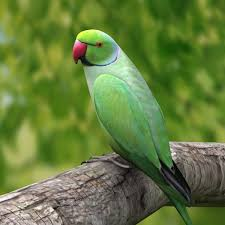
\includegraphics{images (6).jpeg}
    \caption{Parrot}
\end{figure}